\documentclass[11pt,a4paper]{article}

\usepackage[margin=1in]{geometry}
\usepackage{lmodern}
\usepackage[T1]{fontenc}
\usepackage{graphicx}
\usepackage{booktabs}
\usepackage{amsmath,amssymb}
\usepackage{microtype}
\usepackage{xcolor}
\usepackage{hyperref}
\usepackage{caption}
\usepackage{enumitem}
\usepackage[numbers,sort&compress]{natbib}

\hypersetup{
  colorlinks=true,
  linkcolor=black,
  citecolor=black,
  urlcolor=blue!50!black
}

\title{\textbf{RFB--HORN: Learnable oscillatory frequency\\decomposition for compact spoken-digit recognition}}
\author{Samim~A.~Winiger\\
\small Independent researcher}
\date{}

\begin{document}
\maketitle
\begin{center}
\small
\href{https://github.com/samim23/oscnet}{github.com/samim23/oscnet}
\quad$\cdot$\quad July 2026
\end{center}

\begin{abstract}
Speech carries structure across timescales. Inspired by
AudioPrism~\citep{pietras2026audioprism}, we study a small digital stack with
two stages: a learnable \emph{resonator filter bank} (RFB) and a densely
coupled \emph{HORN} (harmonic oscillator recurrent network). Biology is
inspiration only.

On Google Speech Commands digits (v0.02), learnable RFB$\to$dense HORN reaches
$0.76\pm0.02$ clean accuracy at $\sim$7k parameters, while the same RFB
features with a pooled MLP collapse to $0.36\pm0.01$---so
\emph{temporal integration} is load-bearing. Matched sequential controls
(including a GRU) show that oscillation is not the only way to use time---but
on mel features, dense HORN nearly matches a $\sim$3$\times$ larger GRU
($\sim$7k vs.\ $\sim$19k params), and RFB arms retain an additive-noise
advantage under clean training. We also report structure
ablations (equal-frequency $\approx$ chance), learning requirements,
robustness tradeoffs, and nulls (phase, AGC, high$\to$low coupling under our
probe).
\end{abstract}

\section{Introduction}
\label{sec:intro}

Speech encodes information across timescales. Biological hearing is often
described as combining tonotopic decomposition with multi-scale
integration~\citep{pietras2026audioprism}. We treat that description as
\emph{inspiration} for a small digital encoder---not as neuroscience
validation.

AudioPrism~\citep{pietras2026audioprism} established that a \emph{frozen}
cochlear-like resonator bank (PRISM) in front of a HORN unlocks learnability
for small spoken-digit models. We extend that two-stage idea
(Figure~\ref{fig:arch}) with learnable $\{\omega,Q\}$, framed features, and dense
learned coupling, and we include matched sequential controls so gains are not
confused with ``any recurrence helps.''

\paragraph{Contributions.}
\begin{enumerate}[leftmargin=1.4em,itemsep=0.2em]
  \item \textbf{Temporal integration is load-bearing.} Pooled MLP on RFB
  frames fails; framed HORN succeeds.
  \item \textbf{HORN is compact.} At $\sim$7k parameters, mel$\to$dense HORN
  nearly matches a larger non-oscillatory sequential head on clean digits
  (Section~\ref{sec:controls}).
  \item \textbf{RFB structure and learning matter on the RFB path.}
  Equal-frequency banks fail; frozen RFB trails mel; learning $\{\omega,Q\}$
  lifts RFB$\to$HORN (Figure~\ref{fig:bands}).
  \item \textbf{Noise asymmetry.} Clean-trained RFB sequential arms retain
  higher white-noise accuracy than matched mel arms in our protocol.
  \item \textbf{Nulls.} Phase readout, bank AGC, and high$\to$low coupling
  streamlining fail under our probes.
\end{enumerate}

\begin{figure}[t]
  \centering
  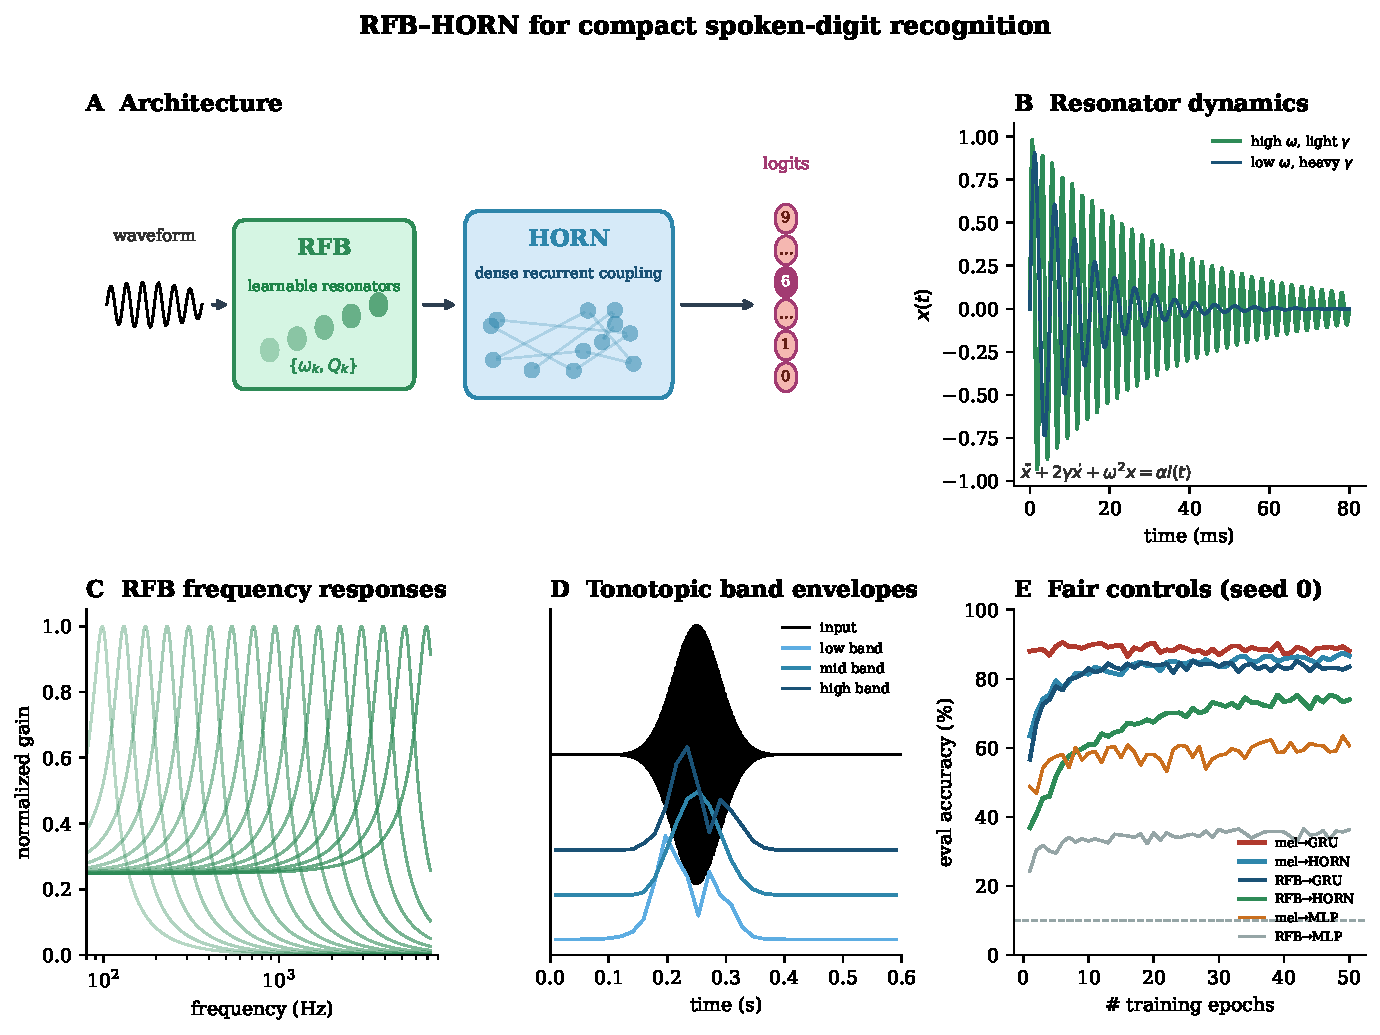
\includegraphics[width=\linewidth]{figures/fig_hero.pdf}
  \caption{\textbf{(A)}~Two-stage stack: learnable RFB into densely coupled
  HORN. \textbf{(B)}~DHO impulse responses. \textbf{(C)}~Log-spaced RFB
  gains. \textbf{(D)}~Tonotopic band envelopes. \textbf{(E)}~Fair-control
  training curves (seed~0): sequential heads dominate pooled MLP; mel leads
  on clean accuracy.}
  \label{fig:arch}
\end{figure}

\section{Related work}
\label{sec:related}

\paragraph{AudioPrism.}
Pietras et al.~\citep{pietras2026audioprism} stack a frozen analytic resonator
bank with a trainable HORN. We cite that as prior art---not as an identical
protocol we claim to beat. Our extensions: learnable $\{\omega,Q\}$, framed
features, dense $W$, classical and sequential controls, robustness, and nulls.

\paragraph{Learnable filterbanks.}
SincNet~\citep{ravanelli2018sincnet} and LEAF~\citep{zeghidour2021leaf} show
constrained learnable fronts help in small-channel / noisy regimes. We use a
driven DHO power response---physics-\emph{shaped}, not hardware.

\paragraph{Controls.}
We report exact trainable parameter counts per arm and compare pooled MLP,
framewise GRU, and HORN under RFB and mel frontends. Dense $W$ adds parameters
relative to fractal-fixed HORN; the default GRU head is larger ($\sim$19k).
Section~\ref{sec:isoparam} adds an iso-parameter GRU ($H{=}34$, $\sim$7k).

\section{Method}
\label{sec:method}

\subsection{Resonator filter bank}
Each band $k$ obeys
\begin{equation}
  \ddot x_k + 2\gamma_k \dot x_k + \omega_k^2 x_k = \alpha_k\, I(t),
  \qquad \gamma_k=\omega_k/(2Q_k).
\end{equation}
Default init: $K{=}32$, $Q{=}4$, 16\,kHz, log-spaced
$f\in[100,7000]$\,Hz, unit-peak $\alpha_k$. Learnable banks optimize bounded
residuals
$\Delta\log\omega_k,\Delta\log Q_k$ with
$\log\omega=\log\omega_0+0.5\tanh(\Delta\log\omega)$ (likewise $Q$), then
sort and clip ($Q\in[0.5,64]$, $\omega$ below $0.9\times$ Nyquist). Gradients
use the frequency-domain DHO power response (not BPTT through an IIR). Features
are $T{=}16$ non-overlapping frames of log-power amplitude
\begin{equation}
  z_{t,k}=\log\!\big(\langle x_k^2\rangle_{\mathrm{frame}\,t}+\varepsilon\big),
\end{equation}
with band-spacing regularizer weight $0.1$ when learning $\{\omega,Q\}$.

\subsection{Heads}
\textbf{MLP.} Two-layer GELU on \emph{mean-pooled} features.\\
\textbf{GRU.} Standard GRU~\citep{cho2014gru} (\texttt{eqx.nn.GRUCell}) over
frames; linear readout on the final state.\\
\textbf{HORN.} Input $u_t=W_{\mathrm{in}}z_t$, recurrent $r_t=W v_t$, and
fixed-dynamics nonlinear oscillators ($\omega_{\mathrm{h}}{=}2\pi/28$,
$\gamma_{\mathrm{h}}{=}0.01$, $\alpha{=}0.04$, $\Delta t{=}1$ per frame):
\begin{align}
  x &\leftarrow x + \Delta t\, v,\\
  v &\leftarrow v + \Delta t\bigl(\alpha\tanh(u_t+r_t)
       -\omega_{\mathrm{h}}^2 x - 2\gamma_{\mathrm{h}} v\bigr),
\end{align}
with linear readout on $x_T$. Trainable: $W_{\mathrm{in}}$, $W$, readout.
Coupling $W$: fractal-fixed, dense, or dense-tonotopic init.

\subsection{Protocol}
\textbf{Data.} Speech Commands v0.02~\citep{warden2018speechcommands} digits
(\texttt{zero}--\texttt{nine}); 16\,kHz, peak-normalized 1.0\,s clips.
Mel uses the full-rate waveform; the RFB frontend uniformly subsamples each
clip to 4096 samples and scales its internal sample rate accordingly (compute
tradeoff; band schedule stays $[100,7000]$\,Hz in that scaled rate).
Official \texttt{validation\_list.txt} and \texttt{testing\_list.txt} are
pooled as the evaluation pool; remaining files form the train pool (speaker
disjoint by construction of those lists). We draw balanced subsamples
$N_{\mathrm{train}}{=}10^4$, $N_{\mathrm{eval}}{=}1200$ with seed-dependent
shuffles; mid-scale confirm uses 4k train. Training uses a fixed 50-epoch
schedule with no early stopping; we report final-epoch evaluation accuracy
(the evaluation pool was also used for iterative inspection during the project).\\
\textbf{Opt.} Adam, batch 64, 50 epochs; lr $3{\times}10^{-3}$ (RFB) or
$10^{-2}$ (mel); four seeds $\{0,1,2,3\}$ unless noted.\\
\textbf{Noise.} Optional train gain $\pm 12$\,dB and, with prob.\ $p$, one of
white / pink ($1/f$) / bandlimited (300--3000\,Hz) noise at
SNR $\mathcal{U}[0,15]$\,dB. Eval noise: independent 10\,dB draws
(same generators) on the evaluation subsample. Unless noted, Table~\ref{tab:controls}
models are \emph{clean-trained} ($p{=}0$).

\section{Experiments}
\label{sec:expts}

Chance $=0.10$. Accuracies are mean$\pm$sample std over seeds.

\subsection{Pooled controls understate temporal heads}
\label{sec:main}

\begin{table}[t]
\centering
\caption{Coupling / pooled-head study (two seeds). Clean is mean$\pm$sample
std; noise columns are seed means. MLP mean-pools frames.}
\label{tab:main}
\small
\begin{tabular}{@{}lrrrrr@{}}
\toprule
Model & Params & Clean & White & Pink & Band \\
\midrule
RFB$\to$dense HORN & 7083 & $0.761{\pm}0.029$ & 0.469 & 0.634 & 0.372 \\
RFB$\to$tonotopic HORN & 7083 & $0.758{\pm}0.017$ & 0.485 & 0.651 & 0.382 \\
RFB$\to$fractal-fixed HORN & 2987 & $0.649{\pm}0.035$ & 0.247 & 0.437 & 0.248 \\
mel$\to$MLP (pooled) & 5514 & $0.608{\pm}0.014$ & 0.398 & 0.491 & 0.391 \\
RFB$\to$MLP (pooled) & 5738 & $0.356{\pm}0.004$ & 0.175 & 0.333 & 0.153 \\
\bottomrule
\end{tabular}
\end{table}

Table~\ref{tab:main} reproduces the early headline: RFB$\to$HORN clears
pooled mel$+$MLP, and pooled MLP on RFB frames collapses. Dense $W$ recovers
$\sim$11 points over frozen fractal structure. This comparison alone cannot
attribute the gain to \emph{oscillation} rather than \emph{sequence use}.

\subsection{Fair sequential controls (four seeds)}
\label{sec:controls}

\begin{table}[t]
\centering
\caption{Fair-control package (10k train, four seeds; clean-trained).}
\label{tab:controls}
\small
\begin{tabular}{@{}llrrr@{}}
\toprule
Frontend & Head & Params & Clean & White 10\,dB \\
\midrule
mel & GRU & 19338 & $\mathbf{0.880{\pm}0.019}$ & $0.381{\pm}0.007$ \\
mel & dense HORN & 6859 & $0.863{\pm}0.008$ & $0.310{\pm}0.055$ \\
RFB learn & GRU & 19562 & $0.836{\pm}0.011$ & $\mathbf{0.646{\pm}0.051}$ \\
RFB learn & dense HORN & 7083 & $0.764{\pm}0.020$ & $0.465{\pm}0.027$ \\
mel & MLP (pooled) & 2762 & $0.600{\pm}0.007$ & $0.378{\pm}0.047$ \\
RFB learn & MLP (pooled) & 5738 & $0.356{\pm}0.009$ & $0.231{\pm}0.053$ \\
\bottomrule
\end{tabular}
\end{table}

Table~\ref{tab:controls} and Figures~\ref{fig:arch} /~\ref{fig:ctrl} clarify
what the architecture is doing:
\begin{itemize}[leftmargin=1.2em,itemsep=0.15em]
  \item Sequential heads (HORN or GRU) dominate pooled MLP.
  \item On clean digits, a larger GRU is slightly ahead; HORN stays close at
  $\sim$1/3 the parameters (mel: $0.86$ vs.\ $0.88$).
  \item RFB sequential arms keep more white-noise accuracy under clean
  training than matched mel arms.
  \item With fair heads, mel remains competitive with RFB on clean digits.
\end{itemize}

\begin{figure}[t]
  \centering
  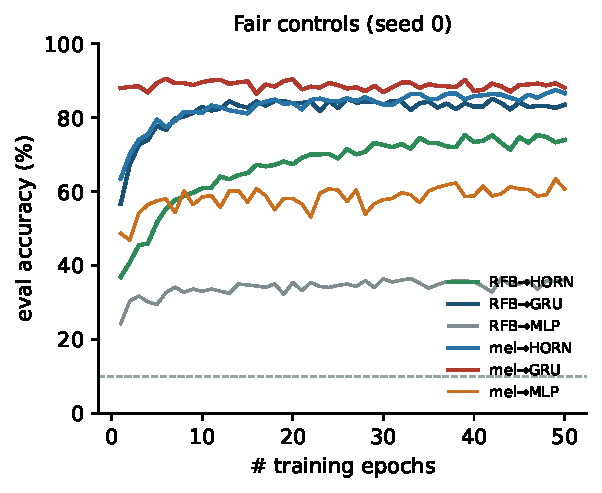
\includegraphics[width=0.85\linewidth]{figures/fig_controls_curves.pdf}
  \caption{Fair-control training curves (seed~0). Sequential heads dominate
  pooled MLP; mel$+$GRU/HORN lead on clean accuracy.}
  \label{fig:ctrl}
\end{figure}

\subsection{Iso-parameter GRU ($\sim$7k)}
\label{sec:isoparam}

\begin{table}[t]
\centering
\caption{Iso-parameter sequential heads (10k train, four seeds; clean-trained).
GRU hidden size $H{=}34$ vs.\ dense HORN $H{=}64$.}
\label{tab:isoparam}
\small
\begin{tabular}{@{}llrrr@{}}
\toprule
Frontend & Head & Params & Clean & White 10\,dB \\
\midrule
mel & GRU ($H{=}34$) & 7218 & $\mathbf{0.873{\pm}0.016}$ & $0.329{\pm}0.088$ \\
mel & dense HORN & 6859 & $0.863{\pm}0.008$ & $0.310{\pm}0.055$ \\
RFB learn & GRU ($H{=}34$) & 7442 & $0.845{\pm}0.010$ & $\mathbf{0.615{\pm}0.018}$ \\
RFB learn & dense HORN & 7083 & $0.764{\pm}0.020$ & $0.465{\pm}0.027$ \\
\bottomrule
\end{tabular}
\end{table}

Matching parameter budgets (Table~\ref{tab:isoparam}) does not reverse the
story: on mel, HORN stays within $\sim$1 point of a $\sim$7k GRU; on RFB, the
iso-parameter GRU still leads on clean accuracy and white-noise robustness.
Compactness remains a HORN strength on the mel path; uniqueness does not.

\subsection{Structure and learning on the RFB path}
\label{sec:structure}

Before learning, Stage~0 (MLP heads) already shows frequency structure
matters:

\begin{center}
\small
\begin{tabular}{@{}lr@{}}
\toprule
Frontend & Accuracy \\
\midrule
mel / STFT / conv1d & $\sim$0.58--0.61 \\
frozen log RFB & $\sim$0.44 \\
equal-frequency RFB & $\sim$0.14--0.16 \\
raw / raw-wide & $\sim$0.13 \\
\bottomrule
\end{tabular}
\end{center}

Four-seed mid-scale confirm: learnable RFB$\to$HORN $0.648\pm0.025$ on digits
and $0.608\pm0.033$ on core-10, vs.\ mel$\to$MLP $0.583\pm0.027$ /
$0.473\pm0.009$ (pooled-head protocol).

\begin{figure}[t]
  \centering
  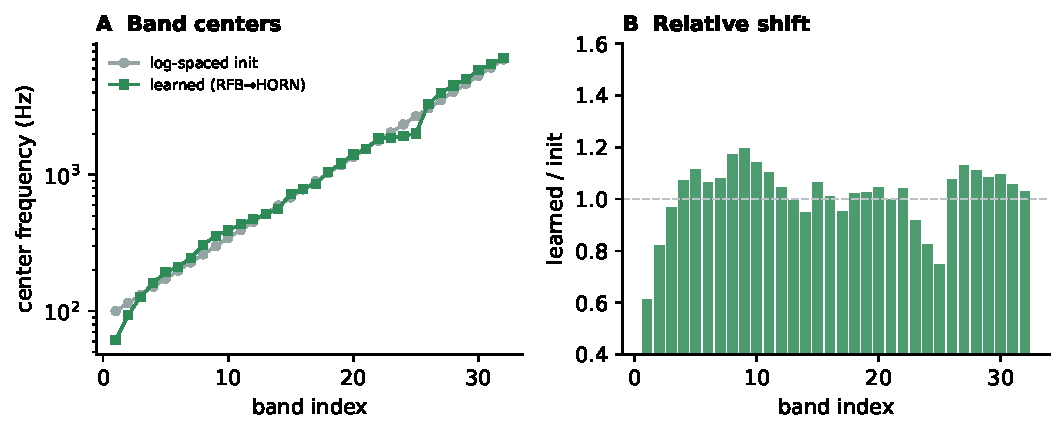
\includegraphics[width=0.92\linewidth]{figures/fig_learned_bands.pdf}
  \caption{Illustrative learned RFB centers after RFB$\to$dense HORN training
  (seed~0). Bands remain roughly log-spaced with mean
  $|\log(\omega/\omega_0)|\approx 0.10$.}
  \label{fig:bands}
\end{figure}

\subsection{Clean vs.\ noise augmentation}
\label{sec:robust}

\begin{figure}[t]
  \centering
  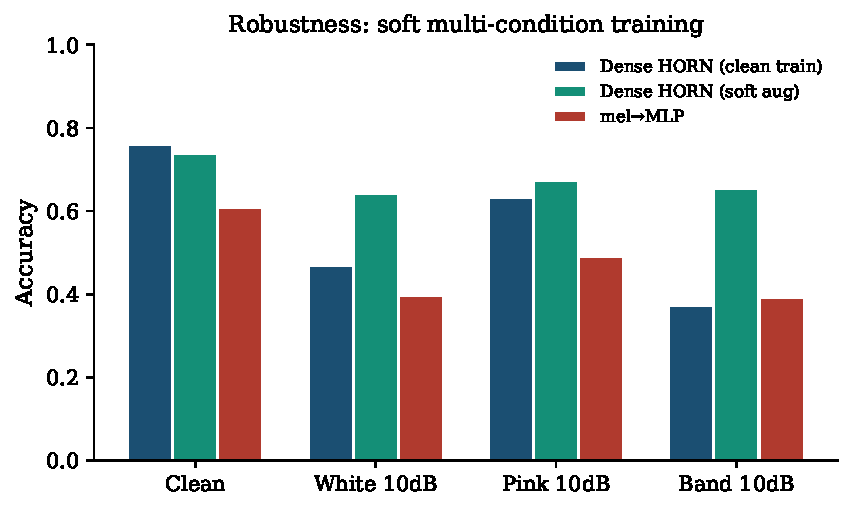
\includegraphics[width=0.92\linewidth]{figures/fig2_robustness.pdf}
  \caption{Soft augmentation trades a little clean accuracy for large
  additive-noise gains (RFB$\to$dense HORN).}
  \label{fig:robust}
\end{figure}

For RFB$\to$dense HORN (two seeds), soft aug ($p{=}0.4$, $\pm 12$\,dB) moves
clean $0.761{\pm}0.029\to0.740{\pm}0.006$ while white 10\,dB rises
$0.469{\pm}0.019\to0.642{\pm}0.035$ (Figure~\ref{fig:robust}). Harder aug
($p{=}0.7$) reaches white $0.678{\pm}0.022$ at a larger clean cost
($0.705{\pm}0.021$).

\subsection{What failed}
\label{sec:nulls}

\paragraph{Relative to AudioPrism-style stories.}
Frozen RFB does not beat mel here; high$\to$low coupling ratios stay
$\approx 1.0$--$1.06$ under our preferred-band probe (Appendix~\ref{app:nulls}).
We do not claim a contradiction of AudioPrism hardware results.

\begin{figure}[t]
  \centering
  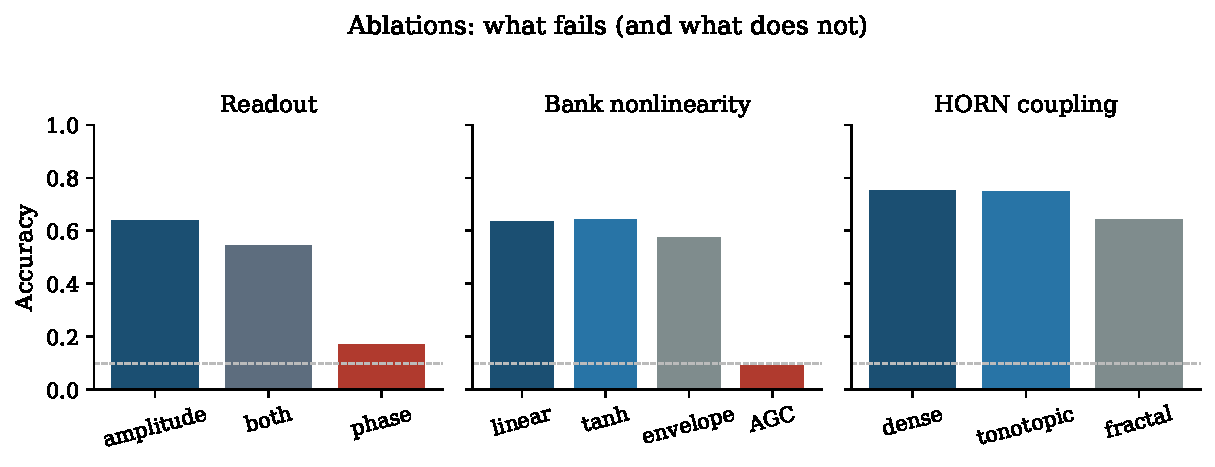
\includegraphics[width=\linewidth]{figures/fig3_ablations.pdf}
  \caption{Ablations: amplitude wins; blunt nonlinearities fail; dense
  coupling beats frozen fractal structure.}
  \label{fig:ablate}
\end{figure}

Additional nulls (Figure~\ref{fig:ablate}): phase-only $\sim$0.18; AGC
$\to$ chance; tonotopic init $\approx$ dense on accuracy without creating
high$\to$low structure.

\section{Discussion}
\label{sec:discuss}

The corrected claim is narrower---and stronger scientifically---than ``RFB beats
mel.'' \textbf{Pooled readouts hide the value of temporal integration.} With a
framed sequential head, mel remains strong on clean digits, while RFB shows a
noise-robustness advantage in our clean-train stress tests. HORN's practical
niche here is \textbf{compact sequence modeling}
(Table~\ref{tab:isoparam})---competitive accuracy at small parameter count,
not unique supremacy over every recurrent alternative.

\paragraph{Limitations.}
Digit-only Speech Commands; pooled val$+$test evaluation subsample (not the
full official test list); evaluation pool was inspected during development
(no held-out final blind test); RFB uses 4096-sample waveform subsampling while
mel does not (Section~\ref{sec:method}); no full 35-class KWS, large SSL, or
tiny-CNN baselines; biological language is inspirational only.

\paragraph{Default recipe (when choosing HORN).}
Learnable RFB or mel frames, dense HORN, $K{=}32$, $H{=}64$, 16 steps; soft
aug if noise robustness matters.

\section{Conclusion}
\label{sec:concl}

Learnable resonator decomposition with oscillatory recurrence is a viable
small spoken-digit encoder when frames are integrated over time. HORN is a
compact sequential head; RFB contributes a noise-robustness role; several
biologically flavored extras fail cleanly. That is a falsifiable extension of
the AudioPrism architectural idea---not a claim of ASR supremacy.

\section*{Acknowledgments}
We thank the AudioPrism authors for a clear architectural target.
Experiments ran on Modal A10G GPUs. AI research agents assisted with
implementation, sweeps, analysis, and drafting under the author's direction;
the author is solely responsible for the scientific claims. Code and CSV
summaries:
\href{https://github.com/samim23/oscnet}{github.com/samim23/oscnet}~\citep{oscnet2026github}.

\bibliographystyle{plainnat}
\bibliography{references}

\appendix
\section{Coupling diagnostics}
\label{app:nulls}
\begin{table}[h]
\centering
\caption{Coupling diagnostics (scale, clean train; two seeds).}
\label{tab:diag}
\small
\begin{tabular}{@{}lccc@{}}
\toprule
Coupling & High$\to$low ratio & Ablate-low drop & Ablate-high drop \\
\midrule
dense & 1.04 & 0.63 & 0.55 \\
dense tonotopic & 1.01 & 0.63 & 0.56 \\
fractal fixed & 1.00 & 0.54 & 0.45 \\
\bottomrule
\end{tabular}
\end{table}

\section{Reproducibility}
\label{app:repro}
\begin{sloppypar}
Sweep entrypoint: \texttt{scripts/modal\_audio\_digit.py}
(\texttt{--sweep-preset}).
Key presets: controls, isoparam, scale, noiseaug, tonotopic
(prefix \textsf{rfb\_plus\_}).
Summaries: \texttt{outputs/analysis/}.
\end{sloppypar}

\end{document}
